

\newpage
\section{Klassendiagramm}

 \subsection{Klassendiagramm}
 \begin{figure}[ht!]
  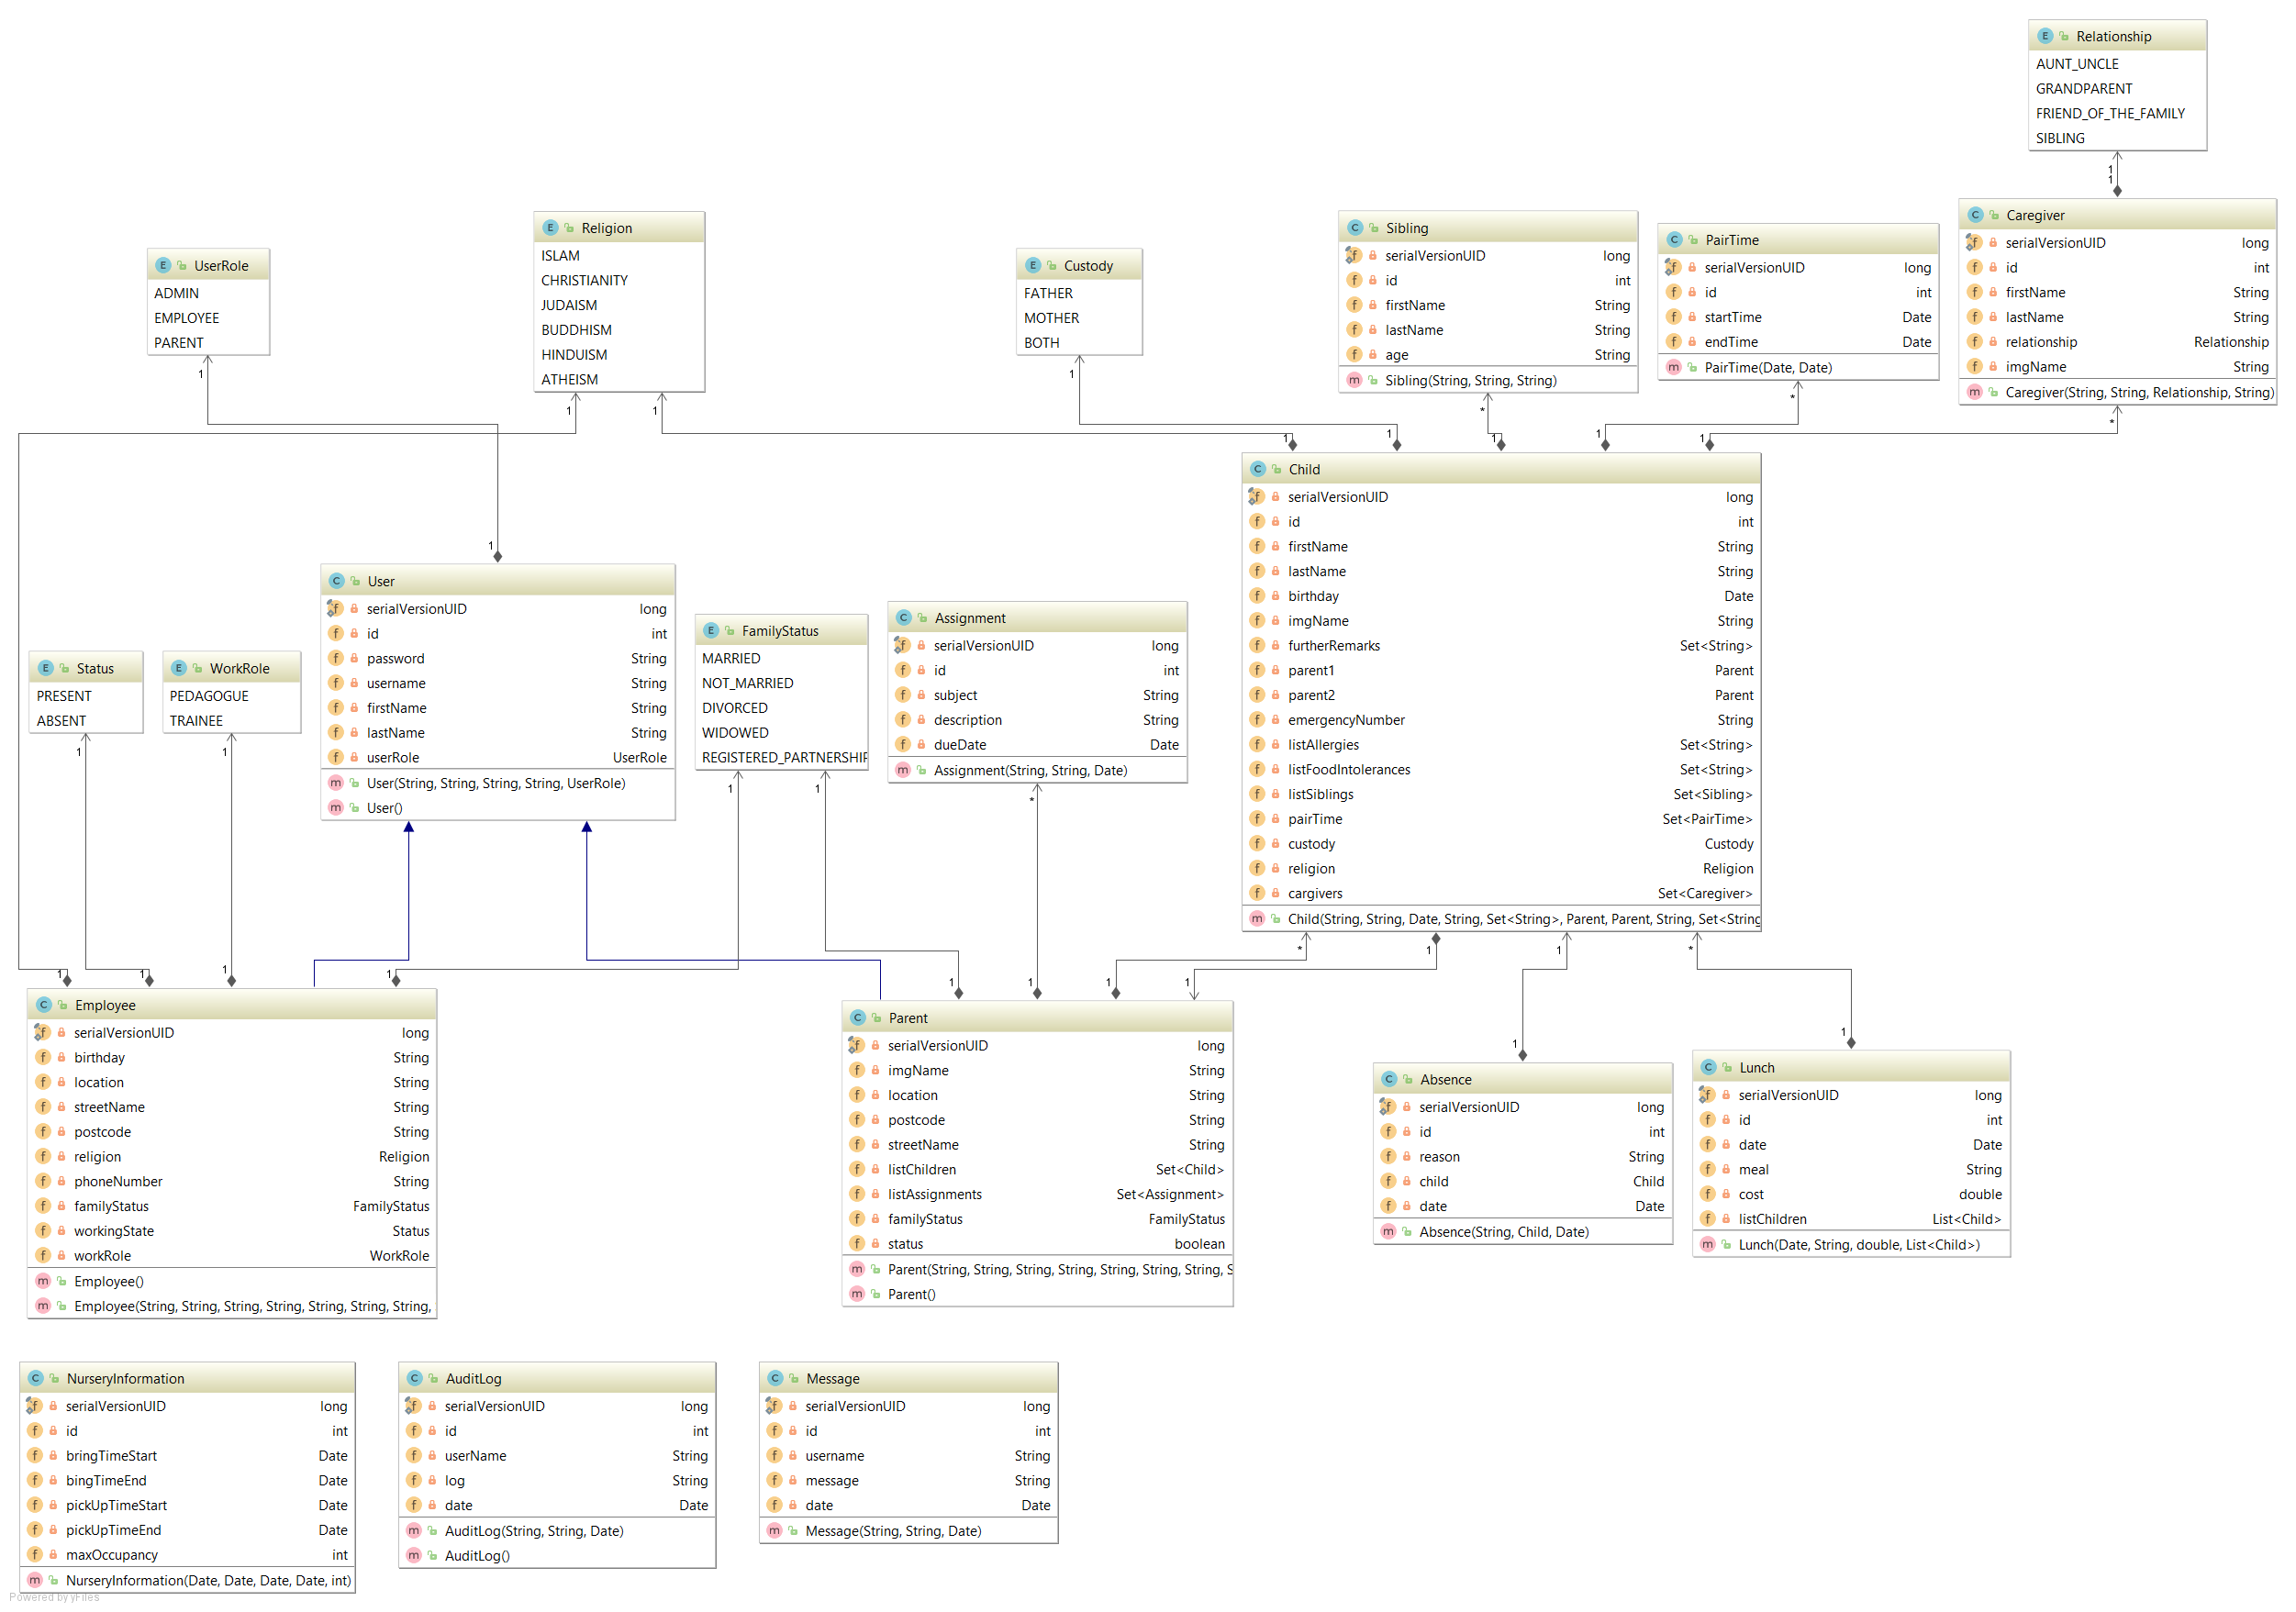
\includegraphics[width = 150mm]{pictures/class_diagram_intellij_bright.png}
 \end{figure}

\newpage
\subsection{Child}
	Haupt-Klasse für alle Kinder die in der Kinderkrippe registriert sind. Zusätzlich zu Attributen wie Namen, Geburtsdatum oder Elternteile sind in dieser Klasse auch Informationen zu Allergien, Nahrungsmittelunverträglichkeiten oder Geschwistern vorhanden. 
\paragraph{Absence}
	Wenn ein Kind an einem regulären Tag von der Kinderkrippe fernbleibt muss dieser Verbleib in dieser Klasse festgehalten werden. Dafür wird der Grund in Form eines Strings abgespeichert und zusätzlich noch das Kind selber und das Datum der Abwesenheit notiert.
\paragraph{Custody}
	Gibt an welche Elternteile (Vater, Mutter oder beide) für die Obhut eines Kindes verantwortlich sind. 
\paragraph{Pairtime}
	Diese Klasse besteht aus einem Paar von java.util.Date. Wir haben diese Klasse erstellt um zum Beispiel Abhol- und Bringzeiten klar darstellen zu können. 
\paragraph{Sibling}
	Sibling ist eine kleinere Version der Child-Klasse. Jede/r Schwester/Bruder ist zwar ebenfalls als Kind in der Kinderkrippe registriert, wird hier aber nur mit dem vollständigen Namen und Alter referenziert um unnötige Datenduplizierung zu vermeiden. 

\subsection{Employee}
	In Employee werden alle Pädagogen und Auszubildenden festgehalten. Pädagogen (Enum WorkRole) haben Zugriff auf alle Daten der Kinder und der Auszubildenden. 
\paragraph{Status}
	Beinhaltet Information über An- und Abwesenheit eines Mitarbeiters. 
\paragraph{WorkRole}
	Gibt an ob ein Mitarbeiter ein Pädagoge oder ein Auszubildender ist.
	
\subsection{Nursery}
\paragraph{AuditLog}
	Im AuditLog werden alle Ereignisse gespeichert die datenbanktechnisch relevant sind. Hierzu gehören erstellen, löschen und editieren von Benutzern. Jeder Eintrag im AuditLog wird mit einem Zeitstempel und dem Benutzer versehen, welcher den Eintrag hervorgerufen hat. 
\paragraph{Lunch}
	Speichert alle nötigen Werte für das tägliche Mittagessen, zu dem die Eltern ihre Kinder anmelden können. Es werden Datum, Mahlzeit, Kosten und die Liste der angemeldeten Kinder vermerkt. Sowohl Mitarbeiter als auch Eltern haben Zugriff auf diese Klasse, wobei nur Mitarbeiter die Werte verändern können.
\paragraph{Message}
	Benutzer können im Messageboard Nachrichten erstellen. Um dies zu ermöglichen verwenden wir "Message" als Hilfsklasse. 
\paragraph{NurseryInformation}
	NurseryInformation beinhaltet die Zeiten an denen Eltern ihre Kinder in die Kinderkrippe bringen und wieder abholen können. Zudem wird noch ein Wert abgespeichert, der die Maximalbelegung der Kinderkrippe anzeigt. 
	
\subsection{User}
User ist die Ausgangsklasse für die Klassen Employee und Parent. Sie bietet grundlegende Attribute wie etwa userName, password, firstName, lastName und die userRole. 
In unserer Implementierung ist ein Admin vorhanden, jedoch nicht als eigene Klasse, da wir datenbanktechnisch in einige Probleme liefen. Es hat sich daher für uns als sinnvoller herausgestellt ihn nur als User mit einer zusätzlichen UserRole zu implementieren. 
\paragraph{UserRole}
Gibt an welcher Position ein Benutzer zugehörig ist (Admin, Employee oder Parent). 
